\section{Threads und Prozesse}
Prozesse sind die Ausführung eines Programms auf dem Prozessor. Jedoch kann ein Prozessor maximal ein Prozess gleichzeitig ausführen. Um Verwirrung zu beseitigen möchte ich darauf hinweisen, dass selbst moderne Prozessoren nicht in der Lage sind mehrere Prozesse auszuführen. Diese ``Illusion'' wird erzeugt, da ein Prozessor(Bauteil) mehre Kerne hat. Diese Kerne sind die eigentlichen Prozessoren. In Zukunft werde ich den Begriff Kerne nutzen um die Unterscheidung zu erleichtern. Um trotzdem mehrere Prozesse gleichzeitig zu bearbeiten, werden den einzelnen Kernen die Prozesse für nur wenige Millisekunden zugeordnet. Diese nennt man auch Virtuelle Threads. Jeder Virtuelle Thread kann einem realem Kern zugeordnet werden. Jedoch wird nicht jeder Process gleich lange einem Kern zugeordnet. Die Prozesse konkurrieren um ihre Zeit. Denn schließlich soll mein Computerspiel nicht die gleiche Zeit bekommen, wie meine Stoppuhr app. Diese wechsel zwischen den einzelnen Prozessen nennt man auch Kontextwechsel. Der Kontext des Kerns ändert sich demnach.

\begin{figure}[h]
    \centering
    \begin{tikzpicture}[auto, thick, node distance=2cm, >=triangle 45]
        \draw
        node at(0,0)[name=start1]{}
        node [sum, name=VThread1, right of=start1]{$V_1$}
        node [sum, name=VThread2, right of=VThread1]{$V_2$}
        node [sum, name=VThread3, right of=VThread2]{$V_3$}
        node [sum, name=VThread4, right of=VThread3]{$V_4$}
        node [sum, name=VThread5, right of=VThread4]{$V_5$}
        node [sum, name=VThread6, right of=VThread5]{$V_6$}
        node [sum, name=VThread7, right of=VThread6]{$V_7$}
        node [sum, name=VThread8, right of=VThread7]{$V_8$};
        \draw
        node at(1.7,-3)[name=start2]{}
        node [block, name=Kern1, right of=start2]{$K_1$}
        node [block, name=Kern2, right of=Kern1]{$K_2$}
        node [block, name=Kern3, right of=Kern2]{$K_3$}
        node [block, name=Kern4, right of=Kern3]{$K_4$};
        \draw[->](VThread1) -- node{} (Kern1.north);
        \draw[->](VThread3) -- node{} (Kern2.north);
        \draw[->](VThread4) -- node{} (Kern3.north);
        \draw[->](VThread7) -- node{} (Kern4.north);
    \end{tikzpicture}
    \caption{Aufteilung von Virtuellen Threads auf Kernel}
\end{figure}

\subsection{Aufbau von Prozessen}

Prozesse müssen jedoch noch ein wenig mehr als nur ein Stück code besitzen, um aktiv zu werden. Generell kann man sagen, dass Prozesse aus 7 Elementen bestehen.
Diese nennt man Prozesskontext. Innerhalb des Prozesskontextes gibt es noch den Hardwarekontext.
\begin{itemize}
    \setlength\itemsep{0pt}
    \item Das auszuführende Programm
    \item Die Daten des Programmes. Umfasst etwa die Globalen variablen.
    \item Einen Stack. Ein Stack funktioniert nach dem push und pop verfahren und speichert die lokalen Variablen für einen schnelleren zugriff.
    \item Kernelstack. Umfasst die Systemaufrufe des Prozesses.
          \begin{itemize}
              \item CPU Register. Kann in den meisten Fällen nur ein Befehl speichern (64bit Prozessor = 64bits im Register)
              \item MMU Register, dass den zugriff auf den Arbeitsspeicher verwaltet.
          \end{itemize}
\end{itemize}

Da ein Prozess viele Kontextwechsel durchleben wird, muss das Betriebssystem bestimmte Register speichern. Dazu gehört aus dem Hardwarekontext:

\begin{itemize}
    \setlength\itemsep{0pt}
    \item Instruction Pointer - Die Speicheradresse des nächsten Befehls.
    \item Instruction Register - Der aktuelle Befehl.
    \item Stackpointer - Speichert das ende des Stacks.
    \item Basepointer - Speicheradresse des aktuellen Elementes im Stack.
    \item Akkumulator - Speichert, Ergebnisse der ALU
\end{itemize}

Dies sind die wichtigsten Informationen, um die Rechenoperationen weiterführen zu können. Das Betriebssystem braucht jedoch noch weitere Informationen über einen Prozess. Diese werden auch Systemkontext genannt. Die wichtigsten davon sind:

\begin{itemize}
    \setlength\itemsep{0pt}
    \item Ort in der Prozesstabelle
    \item PID - Prozessnummer
    \item Prozesszustand
    \item Priorität
    \item Eltern- oder Kindprozesse
    \item Zugriffsrechte - Linux: -20 bis 19; Windows: Rechte werden einzeln zugeteilt
    \item Erlaubte Ressourcenmengen - Bsp. Maximaler RAM verbrauch
    \item Verwendete Dateien - Um zu verhindern, dass mehre Prozesse an einer Datei arbeiten
    \item Zugeordnete Geräte - Maus, Tastatur, ...
\end{itemize}

Mithilfe der Prozesstabelle kann das Betriebssystem die einzelnen Prozesse speichern. In dieser werden Prozesskontrollblöcke gespeichert, welche den Hardwarekontext und Systemkontext beinhaltet. Bei einem Kontextwechsel wird der Prozesskontext aus der Prozesstabelle wieder hergestellt.

\newpage

\subsection{Verwalten der Prozesse}

Jedes Betriebssystem muss einen weg haben, um effektiv die Kontextwechsel der Prozesse durchführen zu können. Dazu wird in den meisten Fällen ein \textit{Warteschlange Prozesse}\ref{Warteschlange Prozesse} verwendet. Auch hat ein Prozess deutlich mehr Zustände als nur \textit{untätig} und \textit{rechnend} in einem modernen Betriebssystem. Dazu wird heutzutage meistens das \textit{Prozessmodell}\ref{Prozessmodell} oder eine modifizierte Variante. Linux als Beispiel verwendet ein \textit{8-Zustands Prozessmodell}, welches das Modell mit einem \textit{kernel rechnend} Zustand erweitert.

\begin{figure}[h]
    \centering
    \begin{tikzpicture}[y=-1cm, scale=0.8]
    \pgfmathsetmacro\start{2}
    \pgfmathsetmacro\endValue{5}
    \draw[very thick, -{Stealth[scale=1.5]}](-2,1.5) -- (\start,1.5);

    %Warteschlange
    \foreach \x in {0,...,\endValue}{
        \filldraw[very thick, draw = black, fill = black!10](\start+\x, 1) rectangle (\start+\x+1, 2);
    }

    \pgfmathsetmacro\middleLine{\start+((\endValue+1)/2)}
    \node[align=center] at (\middleLine, 0.7){\small Warteschlange \footnotesize(bereit)};

    \draw[very thick, -{Stealth[scale=1.5]}](\start+\endValue+1,1.5) -- (\start+\endValue+3,1.5);

    \draw[very thick, draw = black](\start+\endValue+3, 0.7) rectangle (\start+\endValue+3+2.5, 2.3) node[pos=.5] {CPU};

    %Linien
    \pgfmathsetmacro\middleCPU{\start+\endValue+3+1.25}
    \pgfmathsetmacro\endLine{\start+\endValue+1}

    \draw[very thick](\middleCPU, 2.3) -- (\middleCPU, 9);
    \draw[very thick, -{Stealth[scale=1.5]}](-1, 9) -- (-1, 1.5);

    %Entzug der CPU
    \draw[very thick, -{Stealth[scale=1.5]}](\middleCPU, 3) -- (-1, 3) node [midway, above] {\small Entzug \footnotesize (timeout)};

    %Event 1
    \draw[very thick, -{Stealth[scale=1.5]}](\middleCPU, 4.5) -- (\endLine, 4.5) node [midway, above] {\small timeout};
    \foreach \x in {0,...,\endValue}{
        \filldraw[very thick, draw = black, fill = black!10](\start+\x, 4) rectangle (\start+\x+1, 5) node[pos=.5] {\small 1};
    }
    \node[align=center] at (\middleLine, 3.7){\small Warteschlange \footnotesize(blockiert)};
    \draw[very thick](\start, 4.5) -- (-1, 4.5) node [midway, above, align=center] {\small Event 1\\\small eingetreten};

    %Event 2
    \draw[very thick, -{Stealth[scale=1.5]}](\middleCPU, 6.5) -- (\endLine, 6.5) node [midway, above] {\small timeout};
    \foreach \x in {0,...,\endValue}{
        \filldraw[very thick, draw = black, fill = black!10](\start+\x, 6) rectangle (\start+\x+1, 7) node[pos=.5] {\small 2};
    }
    \node[align=center] at (\middleLine, 5.7){\small Warteschlange \footnotesize(blockiert)};
    \draw[very thick](\start, 6.5) -- (-1, 6.5) node [midway, above, align=center] {\small Event 2\\\small eingetreten};

    %Event n
    \draw[very thick, -{Stealth[scale=1.5]}](\middleCPU, 9) -- (\endLine, 9) node [midway, above] {\small timeout};
    \foreach \x in {0,...,\endValue}{
        \filldraw[very thick, draw = black, fill = black!10](\start+\x, 8.5) rectangle (\start+\x+1, 9.5) node[pos=.5] {\small n};
    }
    \node[align=center] at (\middleLine, 8.2){\small Warteschlange \footnotesize(blockiert)};
    \draw[very thick](\start, 9) -- (-1, 9) node [midway, above, align=center] {\small Event n\\\small eingetreten};
\end{tikzpicture}
    \caption{Warteschlangen System\protect\footnotemark}
    \label{Warteschlange Prozesse}
\end{figure}
\footnotetext{Grafik in Anlehnung an \cite{BetriebssystemeKompakt}}
\begin{figure}[h]
    \centering
    \begin{tikzpicture}
    %neu
    \draw[very thick, -{Stealth[scale=1.5]}](7, 1) -- (7, 2);
    \filldraw[very thick, draw = black, fill = black!10](6, 3) rectangle (8, 2) node[pos=.5] {\small neu};

    %bereit
    \draw[very thick, -{Stealth[scale=1.5]}](7, 3) -- (7, 4);
    \filldraw[very thick, draw = black, fill = black!10](6, 5) rectangle (8, 4) node[pos=.5] {\small bereit};
    \draw[very thick, -{Stealth[scale=1.5]}](8, 4.3) -- (11, 4.3) node [midway, below] {\small timeout};
    \draw[very thick, -{Stealth[scale=1.5]}](6, 4.7) -- (3, 4.7) node [midway, above] {\small suspendieren};

    %blockiert
    \draw[very thick, -{Stealth[scale=1.5]}](7, 6.5) -- (7, 5) node [midway, anchor=west, align=center] {\small Ereignis\\\small eingetreten};
    \filldraw[very thick, draw = black, fill = black!10](6, 7.5) rectangle (8, 6.5) node[pos=.5] {\small blockiert};
    \draw[very thick, -{Stealth[scale=1.5]}](6, 7.2) -- (3, 7.2) node [midway, above] {\small suspendieren};
    
    %beendet
    \filldraw[very thick, draw = black, fill = black!10](11, 3) rectangle (13, 2) node[pos=.5] {\small beendet};
    \draw[very thick, -{Stealth[scale=1.5]}](12, 2) -- (12, 1);

    %rechnend
    \draw[very thick, -{Stealth[scale=1.5]}](12, 4) -- (12, 3);
    \filldraw[very thick, draw = black, fill = black!10](11, 5) rectangle (13, 4) node[pos=.5] {\small rechnend};
    \draw[very thick, -{Stealth[scale=1.5]}](11, 4.7) -- (8, 4.7) node [midway, above] {\small dispatch};
    \draw[very thick](11.5, 5) -- (11.5, 7);
    \draw[very thick, -{Stealth[scale=1.5]}](11.5, 7) -- (8, 7) node [midway, above, align=center] {\small Warten auf \\\small Ereignis};
    \draw[very thick](12.5, 5) -- (12.5, 9);
    \draw[very thick](12.5, 9) -- (0, 9) node [midway, above] {\small suspendieren};
    \draw[very thick](0, 9) -- (0, 4.5);
    \draw[very thick, -{Stealth[scale=1.5]}](0, 4.5) -- (1, 4.5);

    %bereit suspendiert
    \filldraw[very thick, draw = black, fill = black!10](1, 5) rectangle (3, 4) node[pos=.5, align=center] {\small bereit\\\small suspendiert};
    \draw[very thick, -{Stealth[scale=1.5]}](3, 4.3) -- (6, 4.3) node [midway, below] {\small aktivieren};

    %blockiert suspendiert
    \filldraw[very thick, draw = black, fill = black!10](1, 7.5) rectangle (3, 6.5) node[pos=.5, align=center] {\small blockiert\\\small suspendiert};
    \draw[very thick, -{Stealth[scale=1.5]}](2, 6.5) -- (2, 5) node [midway, anchor=east, align=center] {\small Ereignis\\\small eingetreten};
    \draw[very thick, -{Stealth[scale=1.5]}](3, 6.8) -- (6, 6.8) node [midway, below] {\small aktivieren};
\end{tikzpicture}
    \caption{7-Zustands Prozessmodell\protect\footnote{eine fußnote}}
    \label{Prozessmodell}
\end{figure}
\footnotetext{Grafik in Anlehnung an \cite{BetriebssystemeKompakt}}

\newpage

Wie in der Einleitung schon angesprochen sind die Zustände \textit{bereit} und \textit{rechnend} die wichtigsten Zustände. Mit diesen alleine könnte ein Betriebssystem funktionieren. Es gäbe dazu dann nur eine Warteschlange, in der sich alle Prozesse des Zustandes \textit{bereit} befinden. Idealer Weise implementiert der \textit{Scheduler}\footnote{Programm zum Managen der Warteschlangen.}  einen Algorithmus, welcher die Priorität der Prozesse berücksichtigt. Wie schon erwähnt muss sich der \textit{Dispatcher}\footnote{Programm zum ausführen der Prozesswechsel.} um noch weitere Zustände kümmern. Diese und ihre Beziehungen sind in Grafik \ref{Prozessmodell} zu finden. Zwei davon währen \textit{neu} und \textit{beendet}. Diese sind für eine größere Flexibilität nützlich. Mit dem \textit{beendet} Zustand, können Informationen nachträglich von einem fertigen Prozess aufgerufen werden. Der Zustand \textit{neu} hat die gemeinsame Funktion mit dem \textit{beendet}-Zustand Ressourcen zu sparen.\newline
Ein Entschiedener Fehler ist es anzunehmen, dass alle Prozesse jederzeit Arbeiten wollen. So könnte ein Programm auf eine Tastatur Eingabe oder andere Ereignisse warten. Um diese Funktionalität bereitstellen zu können gibt es den Zustand \textit{blockiert}. In diesen wechselt ein Prozess nach den berechnen und kann aus diesen sich wieder in die Warteschlange der bereiten Prozesse einordnen. In Grafik \ref{Warteschlange Prozesse} werden unterschiedliche Warteschlangen für unterschiedliche Ereignisse erzeugt. Dieses Vorgehen hat den Vorteil gegenüber einer einzelnen ``blockiert-Warteschlange'', dass häufig genutzte Events wie Tastenanschläge nicht von seltenen Events beeinträchtigt werden.\newline
Da es sehr schnell zu vielen Prozessen kommen kann, wird mit den Zuständen \textit{blockiert suspendiert} und \textit{bereit suspendiert} eine Möglichkeit geschaffen, selten genutzte Prozesse aus dem Arbeitsspeicher in den Massenspeicher\footnote{Spezielle Partitionen auf einer Festplatte. Auch \textit{swap} genannt.} zu verschieben. Wie die Namen schon Implizieren Prozesse in den Zuständen \textit{blockiert} und \textit{bereit} jeweils suspendiert und aktiviert werden. Für zusätzliche Geschwindigkeit, können Prozesse selbst im suspendierten Zustand auf Ereignisse reagieren und von \textit{blockiert suspendiert} in \textit{bereit suspendiert} wechseln. Es gibt demnach ein zweites \captionref{Warteschlange Prozesse} für die suspendierten Prozesse. Dieses beinhaltet keinen zugriff auf die CPU, sondern kann die Prozesse maximal aktivieren und in den Arbeitsspeicher verschieben. \cite{BetriebssystemeKompakt}

\newpage

\subsection{Funktionsweise des Schedulers}
Der \textit{Scheduler} ist ein sehr wichtiges und mächtiges Stück Code. Es managed alle anderen Prozesse eines Betriebssystems. Es kann sich die Frage gestellt werden, wie der \textit{Scheduler} ausgeführt wird. Ist er nur ein weiterer Prozess? Dies würde aber implizieren, dass er sich selber Managen würde. Oder wird er auf einem eigenen CPU Kern ausgeführt? Aber Linux läuft doch auch auf einem einzelnem Kern. Die Antwort liegt in der Natur des Kernels.
\medskip
\newline
Der Kernel ist die niedrigste Instanz mit der höchsten Berechtigung in einem System. Nichts steht neben ihm und der CPU. Jedes Programm muss über den Kernel um etwas machen zu können. Der \textit{Scheduler} ist ein Teil des Kernels. Der Kernel ist jedoch kein einzelner Prozess, welcher immer läuft, sondern eine Art Bibliothek. Ein Programm wendet sich an den Kernel und nicht der Kernel an das Programm. Dementsprechend läuft der \textit{Scheduler} nicht dauerhaft, sondern wird nach einer gewissen Zeit getriggert. Der \textit{Scheduler} wird dabei entweder von einem beendeten Process getriggert oder nach einer Zeitunterbrechung. Die Zeitunterbrechung wird dabei von der CPU durch den \textit{programmable interrupt timer (PIT)} erzeugt und im Kernel durch den \textit{timer interrupt handler} aufgefangen, welcher auch den \textit{Scheduler} startet. Es wird dabei zwischen einem \textit{ticked kernel} und \textit{tickless kernel} unterschieden. Bei dem \textit{ticked kernel} ist der Zeitintervall immer gleich wogegen der des \textit{tickless kernels} dynamisch verändert werden kann.\cite{tickles:Love}
\bigskip
\newline
Der \textit{Scheduler} verwaltet die einzelnen Warteschlangen und entscheidet, wann ein Prozess auf die CPU zugreifen darf. Dabei ist es wichtig die beste Effizienz beizubehalten und trotzdem eine gute Verteilung der Prozesszeit zu ermöglichen. Denn Kontextwechsel sind aufwändig. Bei vielen kleinen Prozessen wird viel Zeit für das speichern der Register und das wiederherstellen eines Prozesses aus der \textit{Prozesstabelle} verwendet. Je länger ein Prozess arbeiten kann, desto effizienter wird die Zeit genutzt. Daher haben sich zwei grundlegende Konzepte des \textit{schedulings} gebildet. Diese Schedulingverfahren sind:
\begin{itemize}
    \item \textit{Nicht-präemptives Scheduling}. Bei diesem ist ein Prozess bis zu seiner Fertigstellung über volle Kontrolle über die CPU. Der \textit{Scheduler} führt erst den Kontextwechsel nach dessen Vollendung aus. Dabei kann es zu Situationen kommen, bei denen ein Prozess sich nicht beendet. Beispielsweise durch eine Endlosschleife in der Programmierung oder der Entwickler setzt bei der Programmierung das \textit{Präemtive Scheduling} voraus.
    \item \textit{Präemtives Scheduling}. Dieses wird seit Windows 3.x und Mac OS8/9 verwendet. Dabei wird nicht auf die Vollendung eines Prozesses gewartet, sondern kann , und wird in den meisten Fällen, der Prozess der CPU vor Beendung entzogen. Der Vorteil ist, dass viele weitere Prozesse ``gleichzeitig'' arbeiten können, ohne dass der Nutzer das ``Einfrieren'' anderer Prozesse erfährt. Der Nachteil dabei ist, dass die Kontextwechsel viel Zeit in Anspruch nehmen. Somit haben die Prozesse weniger Arbeitszeit und die gesamte Leistung der CPU sinkt etwas. Da die Vorteile der größeren Freiheit der leicht verringerten Leistung überwiegen, wird dieses Verfahren in den meisten modernen Betriebssysteme verwendet. \cite{BetriebssystemeKompakt}
\end{itemize}

Auf diesen zwei grundlegenden Systemen haben sich weitere \textit{Scheduling} Verfahren entwickelt, welche das Verwalten der Warteschlange implementieren. Um ein Ideales System zu erschaffen, müssen bestimmte Punkte berücksichtigt werden. Diese lassen sich nicht immer miteinander Vereinbaren und es ist dem Entwickler überlassen, welche er bevorzugt. Diese Kriterien währen wie folgt: \cite{Scheduling:Williams}
\begin{itemize}
    \item Prozessor-Auslastung - Die Prozessor-Auslastung sollte im Idealfall so hoch wie möglich sein. Damit kein Befehlszyklus\footnote{Ein Befehlszyklus ist der kleinste Zeitintervall einer CPU. Befehle können unterschiedlich viele Befehlszyklen brauchen. Je kleiner der Befehlszyklus ist desto höher ist die Herz Anzahl einer CPU} verschwendet wird.
    \item Antwortzeit - Die Zeit, die vergeht, bis die erste Antwort eines Prozesses nach Anfrage ankommt.
    \item Durchlaufzeit - Die Zeit, die vergeht, bis ein Prozess nach Einreichung beendet ist.
    \item Durchsatz - Wie viele Prozesse in einem vorgegebenen Intervall, beendet werden. Der Intervall kann je nach Anwendungsfall variieren.
    \item Wartezeit - Die Zeit, die ein Prozess in der bereit-Warteschlange verbringt, bis er zugriff auf die CPU bekommt.
    \item Fairness - Die Fairness eines Verfahren bestimmt, wie gut kleine und weniger priorisierte Prozesse eine Chance haben Prozesszeit zu erhalten.
\end{itemize}

Im Folgenden werde ich zwei \textit{Scheduling} Verfahren vorstellen.
\newpage
\subsubsection{Completetely Fair Scheduling}
\textit{Completetely Fair Scheduling}\footnote{\textit{Completetely Fair Scheduling (CFS)} wurde 2007 das erste mal von Ingo Molnar im Linux Kernel eingearbeitet.} ist eine, wie der Name schon impliziert, eine Form des \textit{Ideal Fair Scheduling}. Dieses besagt, dass versucht wird die Prozesse gleich lange Arbeiten zu lassen. In den Tabellen \ref{Fair Scheduling} sind vier Prozesse dargestellt. Alle haben die selbe Priorität. In dem Szenario hat jeder Zeit-Quant($Q_1$, $Q_2$, \dots) eine Zeitspanne von 4ms. In den ersten vier Quanten bekommt jeder Prozess 1ms. Ab $Q_4$ sind Prozess B und D abgeschlossen und A und C erhalten somit in $Q_5$ jeweils 2ms. Durch das Prinzip werden alle Prozesse gleich behandelt. \cite{CFS:Rebeiro}
\begin{figure}[h]
    \centering
    \begin{tabular}{| l | l |}
        \hline
        Prozess & Ausführungszeit\\
        \hline
        A & 8ms\\
        \hline
        B & 4ms\\
        \hline
        C & 16ms\\
        \hline
        D & 4ms\\
        \hline
    \end{tabular}
    \begin{tabular}{| x{1em} | x{1em} | x{1em} | x{1em} | x{1em} | x{1em} | x{1em} | x{1em} | x{1em} |}
        \hline
        \rowcolor{black!10}
        & $Q_1$ & $Q_2$ & $Q_3$ & $Q_4$ & $Q_5$ & $Q_6$ & $Q_7$ & $Q_8$\\
        \hline
        \rowcolor{black!20}
        A & 1 & 2 & 3 & 4 & 6 & 8 & &\\
        \hline
        \rowcolor{black!10}
        B & 1 & 2 & 3 & 4 & & & &\\
        \hline
        \rowcolor{black!20}
        C & 1 & 2 & 3 & 4 & 6 & 8 & 12 & 16\\
        \hline
        \rowcolor{black!10}
        D & 1 & 2 & 3 & 4 & & & &\\
        \hline
    \end{tabular}
    \captionof{table}{\textit{Fair Scheduling (FS)}}
    \label{Fair Scheduling}
\end{figure}

Im CFS wird das Prinzip des FS nicht hauptsächlich mit Zeitscheiben gelöst. Es wird das Konzept der \textit{vruntime} eingebracht. \textit{Vruntime} bedeutet dabei, wie lange ein Prozessor bereits ausgeführt wurde. CFS berechnet weiterhin unterschiedliche Zeitscheiben für die PIT, jedoch werden diese zur Maximierung der Effizienz genutzt. Prozesse mit komplexen Rechnungen sind effizienter, wenn sie mehr Zeit ohne Kontextwechsel haben. Andere Prozesse wie Tracker schadet der Kontextwechsel nicht allzu sehr. Der \textit{Scheduler} addiert auf die alte \textit{vruntime} die Zeit($\Delta t$) die der Processor lief. Sollte der Prozess noch nicht abgeschlossen sein, wird die neue \textit{vruntime} in einen Rot-Schwarz Baum eingefügt. Ein Rot-Schwarz Baum ist ein Binärbaum, welcher eine selbst ausgleichende Natur besitzt. Somit beträgt die einfüge Laufzeit $\mathcal{O}(\log n)$. CFS wählt als nächsten Prozess, den mit der geringsten \textit{vruntime} aus. Dabei wird immer ein Pointer auf das kleinste Blatt gehalten, um eine Laufzeit von $\mathcal{O}(1)$ zu erhalten, um den Process mit der kleinsten \textit{vruntime} zu finden. Durch das wählen der kleinsten \textit{vruntime} wird das Prinzip des \textit{Fair Schedulings} eingehalten. \cite{CFS:Rebeiro}
\medskip
\newpage
Das Nutzen der \textit{vruntime} als zentralen Wert hat weitere Vorteile. So können die Prioritäten ohne Umwege eingearbeitet werden. Der CFS verwaltet in der \textit{vruntime} drei unterschiedliche \textit{Scheduling Policies}. \cite{LinuxDoc:Torvalds}
\begin{itemize}
    \item \textbf{SCHED\_NORMAL/SCHED\_OTHER}. Die normale Regel für Prozesse.
    \item \textbf{SCHED\_BATCH}. Für Prozesse, die nicht interaktiv sind und den Arbeitsbereich des Nutzers nicht stören wollen.
    \item \textbf{SCHED\_IDLE}. Die niedrigste Regel für Prozesse und sie werden an wenigsten bevorzugt.
\end{itemize}
SCHED\_NORMAL und SCHED\_BATCH sind zusätzlich von den \textit{nice} Werten abhängig. Die \textit{nice} Werte reichen von -20 bis 19 und repräsentieren die Priorität eines Prozesses. Je kleiner der \textit{nice} Wert, desto höher ist die Priorität\cite{Scheduler:Kerrisk}. Dabei ist der unterschied Linear. Die Verteilung des Prozessors auf zwei Prozesse mit jeweils 11 und 12, währe 55\% und 45\%. Bei Prozessen mit -4 und -5 ist auch 55\% und 45\%. Die neue \textit{vruntime} wird mit Formel \ref{calc_vruntime}\cite{LinuxKernel:Torvalds} berechnet.
\begin{align}
    \text{vruntime} \mathrel{+}= \text{delta\_exec} \cdot \frac{\text{weigth}}{\text{lw.weight}}
    \label{calc_vruntime}
\end{align}
Dabei ist \textit{weigth} mit 1024 oder \textit{nice\_0} definiert. \textit{lw.weigth} ist die Priorität als \textit{weigth}. Dieses kann aus dem Array in dem Listing \ref{core.c}\cite{LinuxKernel:Torvalds} entnommen werden.
\begin{figure}[h]
    \centering      
    \lstset{
    language=C,
    keywordstyle=\color{blue},
    commentstyle=\color{green},
    }
    \begin{tabular}{c}
        \begin{lstlisting}{Latexkernel core.c}
10886 const int sched_prio_to_weight[40] = {
10887 /* -20 */ 88761, 71755, 56483, 46273, 36291,
10888 /* -15 */ 29154, 23254, 18705, 14949, 11916,
10889 /* -10 */ 9548,  7620,  6100,  4904,  3906,
10890 /*  -5 */ 3121,  2501,  1991,  1586,  1277,
10891 /*   0 */ 1024,  820,   655,   526,   423,
10892 /*   5 */ 335,   272,   215,   172,   137,
10893 /*  10 */ 110,   87,    70,    56,    45,
10894 /*  15 */ 36,    29,    23,    18,    15,
10895 };
        \end{lstlisting}
    \end{tabular}
    \captionof{lstlisting}{Linuxkernel core.c{\footnotesize (v5.17-rc3)} \textit{nice} Werte als \textit{weigth}}
    \label{core.c}
\end{figure}
\newpage

\subsubsection{Round Robin}
Das Round Robin(RR) Verfahren ist weitverbreitet. Es wird in abgewandelter Form auch heutzutage in Windows verwendet.\cite{Windows:Lohmann} Das RR \textit{Scheduling} nutzt Zeitquanten. Diese Befinden sich meistens im ein- oder zweistelligen Millisekundenbereich. Jeder Prozess wird nacheinander für die Länge des Zeitquanten ausgeführt und danach dem Prozessor entzogen. Ist der Prozess früher beendet, wird ein neuer Zeitquant eingeleitet. Ist der Prozess nicht beendet, wird er wieder in die Warteschlange am Ende angehängt.\cite[Seite 176f.]{BetriebssystemeKompakt}\\
\begin{figure}[h]
    \centering
    \begin{tabular}{| l | l |}
        \hline
        Prozess & Ausführungszeit\\
        \hline
        \cellcolor{red!20}A & 30ms\\
        \hline
        \cellcolor{blue!20}B & 50ms\\
        \hline
        \cellcolor{green!20}C & 20ms\\
        \hline
        \cellcolor{black!20}D & 30ms\\
        \hline
    \end{tabular}
    \begin{tabular}{|c|c|c|c|c|c|c|c|c|c|c|c|c|c|c|c|c|c|c|c|c|}
        \hline
        \cellcolor{red!20} & \cellcolor{red!20} & \cellcolor{blue!20} & \cellcolor{blue!20} & \cellcolor{green!20} & \cellcolor{green!20} & \cellcolor{black!20} & \cellcolor{black!20} & \cellcolor{red!20} & \cellcolor{blue!20} & \cellcolor{blue!20} & \cellcolor{black!20} & \cellcolor{blue!20}\\
        \hline
        \multicolumn{1}{l}{} & \multicolumn{2}{c}{\tiny 20} & \multicolumn{2}{c}{\tiny 40} & \multicolumn{2}{c}{\tiny 60} & \multicolumn{2}{c}{\tiny 80} & \multicolumn{2}{c}{\tiny 100} & \multicolumn{2}{c}{\tiny 120}\\
    \end{tabular}
    \caption{Round Robin Beispiel}
    \label{RoundRobin}
\end{figure}

In \ref{RoundRobin} werden vier Prozesse in der vorgegebenen Reihenfolge abgearbeitet. Die Zeitquanten in dem Beispiel sind 20ms lang. Prozess C benötigt nur ein Zeitquanten und wird beendet. Prozesse A und D benötigen 1.5 Zeitquanten. Sie arbeiten beim Zweiten mal nur 10ms und der nächste Prozess kann nachrücken. Prozess B benötigt am meisten Zeit und wird drei mal ausgeführt. Erst beim dritten mal kann er beendet werden.
\medskip
\newline
Das Round Robin Verfahren kann noch mit Prioritäten erweitert werden. Dieses werde ich am Beispiel des \textit{Schedulers} von Windows erklären. Windows verwendet ein Prioritätengesteuertes \textit{Scheduling}\footnote{Die Prioritäten von Windows reichen dabei von 0 bis 31}. Das RR Verfahren wird dabei immer auf die selbe Priorität angewendet. Die höhere Priorität wird immer bevorzugt. Dazu wird für jede Priorität eine eigene Warteschlange angelegt. Um das verhungern eines Prozesses zu verhindern, nutzt Windows noch Variable Prioritäten. Bei den Variablen Prioritäten hat Windows noch die Möglichkeit selber zu ermitteln welche Prozesse wichtiger sind.\cite[Folie 9-12]{Windows:Lohmann}
\medskip
\newline
Mit dem Round Robin Verfahren kann grundsätzlich eine Faire Umgebung geschaffen werden. Werden jedoch Prioritäten ohne Variation bevorzugt, kann es zu einem Unfairen System werden. Auch sind I\/O-lastige\footnote{I\/O = Input\/Output. Ein Prozess wartet z.B. auf eine Eingabe des Benutzers.} Prozesse benachteiligt. Sie benötigen selber nur wenig Ausführungszeit, müssen aber für das reibungslose Funktionieren häufiger Zugriff auf den Prozessor erhalten. Im Round Robin \textit{Scheduling} müssen sie warten bis Rechenintensive Prozesse den Zeitquanten vollständig verbrauchen, bevor sie wieder an der Reihe sind.

\subsection{Threads}\label{Threads}
In Modernen Computer Systemen gibt es noch Threads neben Prozessen. Threads sind dabei deutlich häufiger vertreten als Prozesse. Auf meinem Computer laufen durchschnittlich 20x mehr Threads als Prozesse. Dies liegt daran, dass Threads als Prozess eines Prozesses gesehen werden. Ein Programm ist nur ein Prozess kann aber aber viele eigene Threads besitzen. Die Funktionalität von Threads unterscheidet sich nicht viel von Prozessen. Sie werden im \textit{Scheduler} gleich behandelt und es gibt nur geringe Unterschiede bei dem Kontextwechsel.
\medskip
\newline
Threads haben jedoch ein paar Besonderheiten gegenüber Prozessen. Denn im Gegensatz zu Prozessen, welche unabhängig voneinander Laufen, haben Threads diese Beschränkung nicht. Dies liegt daran, dass Threads auf den Stack des Prozesses zugreifen können. Threads teilen sich somit die globalen Variablen des Prozesses, speichern aber eigene lokale Variablen im eigenen Stack. Wegen diesem Prinzip können mehrere Threads mit dem selben Code arbeiten, ohne sich gegenseitig zu behindern.\cite{Threads:Williams}
\begin{figure}[h]
    \centering
    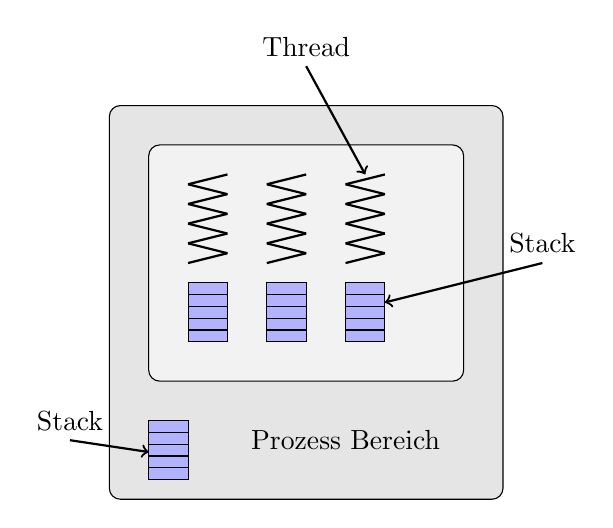
\begin{tikzpicture}[scale=0.5]
    \draw[rounded corners, fill=black!10] (0, 0) rectangle (10, 10){};
    \draw[rounded corners, fill=black!5] (9,9) rectangle (1, 3);

    \foreach \s in {0, 0.3, ..., 1.5}{
        \draw[fill=blue!30] (1, 0.5+\s) rectangle (2, 0.5+\s+0.3);
    }

    \foreach \s in {0, 0.3, ..., 1.5}{
        \draw[fill=blue!30] (2, 4+\s) rectangle (3, 4+\s+0.3);
    }
    \foreach \s in {0, 0.3, ..., 1.5}{
        \draw[fill=blue!30] (4, 4+\s) rectangle (5, 4+\s+0.3);
    }
    \foreach \s in {0, 0.3, ..., 1.5}{
        \draw[fill=blue!30] (6, 4+\s) rectangle (7, 4+\s+0.3);
    }
    
    \foreach \t in {0, 0.5, ..., 1.5}{
        \draw[thick] (2, 6+\t) -- (3, 6+\t+0.25);
        \draw[thick] (3, 6+\t+0.25) -- (2, 6.5+\t);
    }
    \draw[thick] (2, 6+2) -- (3, 8.25);

    \foreach \t in {0, 0.5, ..., 1.5}{
        \draw[thick] (4, 6+\t) -- (5, 6+\t+0.25);
        \draw[thick] (5, 6+\t+0.25) -- (4, 6.5+\t);
    }
    \draw[thick] (4, 6+2) -- (5, 8.25);
    
    \foreach \t in {0, 0.5, ..., 1.5}{
        \draw[thick] (6, 6+\t) -- (7, 6+\t+0.25);
        \draw[thick] (7, 6+\t+0.25) -- (6, 6.5+\t);
    }
    \draw[thick] (6, 6+2) -- (7, 8.25);

    \draw[thick, ->] (5, 11) -- (6.5, 8.25);
    \node[] at (5, 11.5){Thread};

    \draw[thick, ->] (-1, 1.5) -- (1, 1.2);
    \node[] at (-1, 2){Stack};

    \node[] at (6, 1.5){Prozess Bereich};

    \draw[thick, ->] (11, 6) -- (7, 5);
    \node[] at (11, 6.5){Stack};
\end{tikzpicture}
    \caption{Threads}
\end{figure}
\\Threads werden als teil eines Prozesses betrachtet. Deswegen sind sie viel Leichtgewichtiger und können schneller erstellt und beendet werden. Zusätzlich werden Threads in zwei Kategorien unterteilt.
\begin{itemize}
    \item Nutzer Level Threads. Diese werden mithilfe einer Thread-library implementiert und sind unabhängig von dem Betriebssystem. Folgend können Nutzer Level Threads auch auf einem System ohne unterstütztem Multiprozessing in Betrieb genommen werden. Außerdem ist das Management von vielen Threads schneller, da keine Systemaufrufe getätigt werden müssen.
    \item Kernel Level Threads. Diese werden vom Betriebssystem implementiert und auch von diesem verwaltet. Dadurch ergeben sich Vorteile, wie auch Nachteile. Ein Vorteil wäre, dass Prozesse mit einer hohen Thread Anzahl bevorzugt werden könnten. Der Nachteil ist, dass die Verwaltung auf Kernel Ebene deutlich Intensiver ist. Auch muss für jeden Thread ein einzelner Kontrollblock erstellt werden. \cite{Threads:Dusey}
\end{itemize}
\subsection{Threads in Java}
In Java sind die Threads auf dem Kernel Level implementiert. In Versionen vor 1.2(1998) gab es die so genannten grünen Threads. Diese waren Nutzer Level Threads von der Java VM. Der Vorteil durch das Modernere Modell, ist dass die gesamte CPU genutzt werden kann. Ein Prozess mit mehreren Threads kann somit alle vorhandenen CPU Kerne benutzen. Im alten Modell wurde dies über Umwege gelöst. So wurden ein paar Kernel Level Threads erstellt, welche dann die grünen Threads zugewiesen bekamen.\cite{Threads:Cox}
\subsubsection{Implementation in Java}
Threads werden in java mithilfe der \textit{java.lang.Thread} Klasse verwirklicht. Es wird dabei zwischen zwei unterschiedlichen Implementierungen unterschieden.
\smallskip
\newline
\textbf{extends Thread:} Bei dieser Methode wird eine Klasse erstellt, welche die Thread Klasse erweitert. Der Vorteil dieses Vorgehens ist, dass alle Einstellungen innerhalb der neuen Klasse getätigt werden können.\cite{Java:Thread}
\lstset{
language=Java,
keywordstyle=\color{blue},
commentstyle=\color{green},
basicstyle=\linespread{0.8}\small,
}
\begin{figure}[h]
\begin{lstlisting}{extends Thread}
public class SimpleThread extends Thread {

    public SimpleThread(){
        super();
        //settings
        setPriority(Thread.NORM_PRIORITY);
    }

    @Override
    public void run(){
        System.out.println("Im Running");
    }

    public static void main(String[] args){
        SimpleThread t = new SimpleThread();
        t.start();
    }
}
\end{lstlisting}
\captionof{lstlisting}{mit Thread erweitern}
\end{figure}
\\Das Vorgehen hat seine Probleme. Denn es wird nicht die \textit{run()} Methode von Thread überschrieben, sondern die von Runnable, welches von Thread implementiert wird. Wenn die Thread Klasse erweitert wird, kann man keine weiteren Klassen erweitern. Um ein solches Problem zu lösen kann auf die zweite Möglichkeit zurückgegriffen werden.
\smallskip
\newline
\textbf{implements Runnable:}Bei dieser Methode wird nicht ein selbständiger Thread erschaffen. Das Interface Runnable hat nur eine Methode. Die \textit{run()} Methode.\cite{Java:Runnable} Um einen Thread zu starten, muss ein Thread Object erschaffen werden, welche im Konstruktor ein Object des interfaces Runnable erwartet.
\begin{figure}[h]
\begin{lstlisting}
public class SimpleRunnable implements Runnable{
    public SimpleRunnable(){

    }

    @Override
    public void run(){
        System.out.println("Im Running");
    }

    public static void main(String[] args){
        SimpleRunnable r = new SimpleRunnable();
        Thread t = new Thread(r);
        t.start();
    }
}
\end{lstlisting}
\captionof{lstlisting}{Runnable implementieren}
\end{figure}
\\Der Vorteil dieses Vorgehen ist, dass Runnable Leichtgewichtiger ist und erst bei Ausführung ein Thread Object erschaffen wird. Auch ist die seperierung zwischen ``Aufgabe'' und ``Bearbeiter'' sinvoll. Man erhält eine große Flexibilität. Die Funktionen des einstellen eines Threads gegen auch nicht verloren. Die Methoden wie \textit{setPriority()} sind public.\cite{Java:Thread} Ein weiterer wichtioger Punkt ist, dass Runnables in einem ThreadPool verwendet werden können.

\subsubsection{Thread pool}
Ein Thread Pool ist wie eine zweite CPU nur in Software. Es gibt eine Warteschlange und eine festgelegte Anzahl an Threads, welche arbeiten. Der Unterschied dabei ist, dass die Warteschlange nicht aus Threads besteht, sondern aus ``Runnables''. Diese werden auch nur ein einziges Mal ausgeführt und dabei nicht unterbrochen. Auch wird die Warteschlange chronologisch abgearbeitet. Ein Thread pool hat somit ein \textit{nicht-präemtives Scheduling}, welches mit dem \textit{first in first out} Verfahren arbeitet.\newpage
\begin{figure}[h]
    \begin{tikzpicture}
    \foreach \q in{0,0.5,...,4}{
        \filldraw[very thick, draw=black, fill=black!5](0+\q, 7) circle (0.5cm);
    }
    \draw[very thick](4, 7) -- (5.7+4, 7);
    \draw[very thick, -{Stealth[scale=1.5]}](5.7+4, 7) -- (5.7+4, 5.3);
    \filldraw[very thick, draw=black, fill=black!5](4, 7) circle (0.5cm) node[align=center] {$R_n$};

    \foreach \x in {0,1.6,...,8}{
        \filldraw[very thick, draw=black, fill=black!10](5.7+\x, 3.7) rectangle (7.3+\x, 5.3);
        \filldraw[very thick, draw=black, fill=black!5](6.5+\x, 4.5) circle (0.5cm);
    }

    \foreach \q in{0,0.5,...,4}{
        \filldraw[very thick, draw=black, fill=black!5](0+\q, 2) circle (0.5cm);
    }
    \draw[very thick](5.7+4, 3.7) -- (5.7+4, 2);
    \draw[very thick, -{Stealth[scale=1.5]}](5.7+4, 2) -- (4.5, 2);
    \filldraw[very thick, draw=black, fill=black!5](4, 2) circle (0.5cm) node[align=center] {$R_n$};
\end{tikzpicture}
    \caption{Thread pool}
\end{figure}
In einem Thread pool werden die Aufgaben als ``Runnable'' Object verwaltet. Eine bestimmte Anzahl an Threads arbeiten und erhalten immer neue ``Runnables''. Durch dieses Verfahren, muss nicht für jede Aufgabe ein neuer Thread erstellt werden. Auch ist ein Thread pool effizienter. Wenn viel berechnet werden muss, ist es besser weniger aktive Threads zu benutzten. Würde mann alle Aufgaben gleichzeitig starten, müsste der \textit{System Scheduler} die Threads verwalten. Es würden somit viel mehr Kontextwechsel stattfinden, bis alle Aufgaben abgearbeitet sind. Daher ist eine optimale Größe eines Thread pools in der Größenordnung der vorhandenen Kerne.\cite{ThreadPool:Java}

\subsubsection{Thread sicherheit}
\begin{center}
    \textit{
        [...]That the concept [of thread safety] itself is completely vague and essentially means nothing more than ``behaves correctly in some situations''[...]
    } - Eric Lippert \cite{Threads:Lippert}
\end{center}

Wie Herr Lippert in seinem Artikel bereits klarstellt, ist Thread sicherheit kein besonders kleines Thema. Auch ist Thread sicherheit immer im Auge des Betrachters. Es kommt immer auf die Situation an. Ist etwas in diesem speziellen Szenario Thread sicher? Denn eine allumfangende Thread sicherheit kann in den meisten Fällen nicht erreicht werden. Darum werde ich mich auf einen wichtigen Bereich der Thread sicherheit beschränken.
\medskip
\newline
Wie in Kapitel \ref{Threads} beschrieben, haben Threads einen gemeinsamen globalen Speicher. Das Problem dessen tritt auf, wenn mehrere Threads gleichzeitig auf die selben Speicheradresse zugreifen. Ein simples Beispiel ist, dass erhöhen einer Zahl. Diese Situatuion tritt auch in meinem Programm, siehe Kapitel \ref{Programm}, auf. Dabei versuchen mehrere Threads den selben Integer zu erhöhen. Das Ergebnis ist, dass trotz 2000x erhöhen im Integer nur 1800 gespeichert ist. Um das Problem zu verstehen werde ich erklären, wie ein Integer erhöht wird.\\
Ein Integer wird nicht an seinem Speicherort geändert. Die Bytes werden erst in den Prozessor geladen und dann mit dem gewünschten Wert addiert. Der alte Wert wird mit dem neuen Wert aus dem Register überschrieben. Im Falle von vielen Threads fetcht\footnote{Deutsch: bringen - Ein Programm ließt Daten.} sich ein Thread den Wert $W_1 = 500$. Thread zwei, welcher kurz nach Thread eins gestartet wurde, fetcht auch den Wert $W_2 = 500$. Beide addieren ihren Teil und erhalten $W_3 = 501$ und $W_4 = 501$. Beide Werte werden anschließend nacheinander auf den alten Wert geschrieben. Wurde somit der Wert zwei mal erhöht, ist aber im Ergebnis nur um eins gestiegen.\cite{ThreadInterference:Oracle}\\
Um solches Verhalten zu vermeiden, gibt es in Java das Schlüsselwort \textit{synchronized}. Es beschrenkt den Zugriff auf eine Methode oder code Abschnitt auf nur einen Thread. Alle anderen Threads müssen auf das beenden des vorherigen warten. Das Beispiel würde als Thread sichere Version wie folgt aussehen: \cite{SynchronizedMethods:Oracle}
\begin{figure}[h]
    \begin{lstlisting}
public class ThreadSafe{

        int counter=0;

        public synchronized void increase(){
            counter++;
        }
}
    \end{lstlisting}
    \captionof{lstlisting}{Thread sicher}
\end{figure}